
% !TEX root = DesignDocument.tex

\chapter{Design  and Implementation}

\section{Systems Goals}
Briefly describe the overall goals this system plans to achieve.
These goals are typically provided by the stakeholders.  This is not
intended to be a detailed requirements listing.  Keep in mind that
this section is still part of the Overview.

\section{System Overview and Description}
Provide a more detailed description of the major system components
without getting too detailed.  This section should contain a
high-level block and/or flow diagram of the system highlighting the
major components.  See Figure~\ref{systemdiagram}.  This is a floating
figure environment.  \LaTeX\ will try to put it close to where it was
typeset but will not allow the figure to be split if moving it can not
happen.  Figures, tables, algorithms and many other floating
environments are automatically numbered and placed in the appropriate
type of table of contents.  You can move these and the numbers will
update correctly.

\begin{figure}[tbh]
\begin{center}
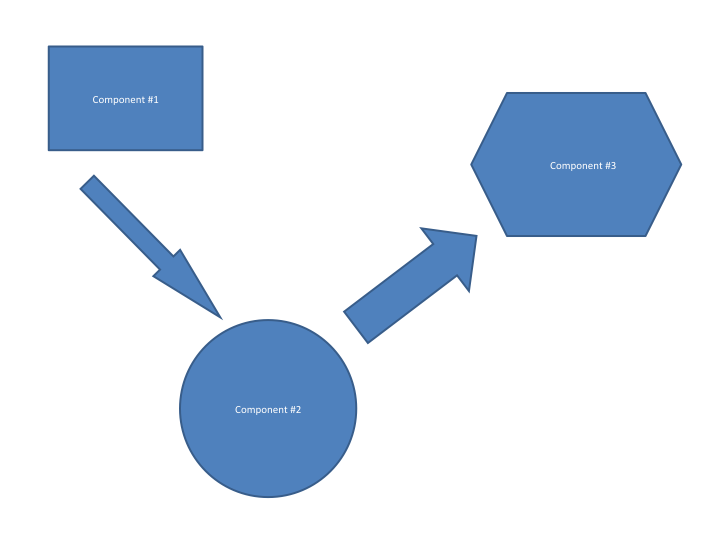
\includegraphics[width=0.75\textwidth]{./diagram}
\end{center}
\caption{A sample figure .... System Diagram \label{systemdiagram}}
\end{figure}

\subsection{Major System Component \#1}
Describe briefly the role this major component plays in this system. 

\subsection{Major System Component \#2}
Describe briefly the role this major component plays in this system. 

\subsection{Major System Component \#3}
Describe briefly the role this major component plays in this system. 


\section{Technologies Overview}
This section should contain a list of specific technologies used to
develop the system.  The list should contain the name of the
technology, brief description, link to reference material for further
understanding, and briefly how/where/why it was used in the system.
See Table~\ref{somenumbers}.  This is a floating table environment.
\LaTeX\ will try to put it close to where it was typeset but will not
allow the table to be split.

\begin{table}[tbh]
\caption{A sample Table ... some numbers. \label{somenumbers}}
\begin{center}
\begin{tabular}{|r|l|}
  \hline
  7C0 & hexadecimal \\
  3700 & octal \\ \cline{2-2}
  11111000000 & binary \\
  \hline \hline
  1984 & decimal \\
  \hline
\end{tabular}
\end{center}
\end{table}


 \section{Architecture and System Design}
This is where you will place the overall system design and the architecture.   This section will be very detailed and should be image rich.  There is the old phrase {\it a picture is worth a thousand words}, in this class it could be worth hundreds of points (well if you sum up over the entire team).   One needs to enter the design and why a particular design has been done.   THIS IS THE CORE OF THE COURSE.    
 
 
 {\it It is important for you to say why as much as what.   }
 
   \subsection{Design Selection}
 Failed designs, design ideas, rejected designs here.
 
 \subsection{Data Structures and Algorithms}
 Describe the special data structures and any special algorithms.
 
 \subsection{Data Flow}
 
 \subsection{Communications}
 
 \subsection{Classes}
 
 \subsection{UML}
 
 \subsection{UX}
 
 \subsection{UI}
 
 \subsection{MVVM, etc}

\section{Major Component \#1 }

{\bf If the following makes sense, use this outline, if not then modify the outline}


This section is used to describe the design details for each of the major components 
in the system.    Note that this chapter is critical for all tracks.  Research tracks would do experimental design here where other tracks would include the engineering design aspects.    This section is not brief and requires the necessary detail that 
can be used by the reader to truly understand the architecture and implementation 
details without having to dig into the code.    Sample algorithm:  Algorithm~\ref{alg1}.  This algorithm environment is automatically placed - meaning it floats.   You don't have to worry about placement or numbering.  

\begin{algorithm} [tbh]                     % enter the algorithm environment
\caption{Calculate $y = x^n$}          % give the algorithm a caption
\label{alg1}                           % and a label for \ref{} commands later in the document
\begin{algorithmic}                    % enter the algorithmic environment
    \REQUIRE $n \geq 0 \vee x \neq 0$
    \ENSURE $y = x^n$
    \STATE $y \Leftarrow 1$
    \IF{$n < 0$}
        \STATE $X \Leftarrow 1 / x$
        \STATE $N \Leftarrow -n$
    \ELSE
        \STATE $X \Leftarrow x$
        \STATE $N \Leftarrow n$
    \ENDIF
    \WHILE{$N \neq 0$}
        \IF{$N$ is even}
            \STATE $X \Leftarrow X \times X$
            \STATE $N \Leftarrow N / 2$
        \ELSE[$N$ is odd]
            \STATE $y \Leftarrow y \times X$
            \STATE $N \Leftarrow N - 1$
        \ENDIF
    \ENDWHILE
\end{algorithmic}
\end{algorithm}
Citations look like~\cite{Choset:2005:PRM, arkin2009governing, lavalle2006}  and~\cite{wiki:asimo,lumelsky:1987, nolfi2000evolutionary}.  These are done automatically.  Just fill in the database {\tt designrefs.bib} using the same field structure as the other entries.  Then pdflatex the document, bibtex the document and pdflatex twice again.  The first pdflatex creates requests for bibliography entries.
The bibtex extracts and formats the requested entries.  The next pdflatex puts them in order and assigns labels.  The final pdflatex replaces references in the text with the assigned labels.
The bibliography is automatically constructed.  
 


\subsection{Technologies  Used}
This section provides a list of technologies used for this component.  The details 
for the technologies have already been provided in the Overview section. 

\subsection{Component  Overview}
This section can take the form of a list of features. 

\subsection{Phase Overview}
This is an extension of the Phase Overview above, but specific to this component. 
 It is meant to be basically a brief list with space for marking the phase status. 

\subsection{ Architecture  Diagram}
It is important to build and maintain an architecture diagram.  However, it may 
be that a component is best described visually with a data flow diagram. 


\subsection{Data Flow Diagram}
It is important to build and maintain a data flow diagram.  However, it may be 
that a component is best described visually with an architecture diagram. 


\subsection{Design Details}
This is where the details are presented and may contain subsections.   Here is an example code listing:
\begin{lstlisting}
#include <stdio.h>
#define N 10
/* Block
 * comment */
 
int main()
{
    int i;
 
    // Line comment.
    puts("Hello world!");
 
    for (i = 0; i < N; i++)
    {
        puts("LaTeX is also great for programmers!");
    }
 
    return 0;
}
\end{lstlisting}
This code listing is not floating or automatically numbered.  If you want auto-numbering, but it in the algorithm environment (not algorithmic however) shown above.



\section{Major Component \#2 }

\subsection{Technologies  Used}
This section provides a list of technologies used for this component.  The details 
for the technologies have already been provided in the Overview section. 

\subsection{Component  Overview}
This section can take the form of a list of features. 

\subsection{Phase Overview}
This is an extension of the Phase Overview above, but specific to this component. 
 It is meant to be basically a brief list with space for marking the phase status. 

\subsection{ Architecture  Diagram}
It is important to build and maintain an architecture diagram.  However, it may 
be that a component is best described visually with a data flow diagram. 


\subsection{Data Flow Diagram}
It is important to build and maintain a data flow diagram.  However, it may be 
that a component is best described visually with an architecture diagram. 


\subsection{Design Details}
This is where the details are presented and may contain subsections. 


\section{Major Component \#3 }

\subsection{Technologies  Used}
This section provides a list of technologies used for this component.  The details 
for the technologies have already been provided in the Overview section. 

\subsection{Component  Overview}
This section can take the form of a list of features. 

\subsection{Phase Overview}
This is an extension of the Phase Overview above, but specific to this component. 
 It is meant to be basically a brief list with space for marking the phase status. 

\subsection{ Architecture  Diagram}
It is important to build and maintain an architecture diagram.  However, it may 
be that a component is best described visually with a data flow diagram. 


\subsection{Data Flow Diagram}
It is important to build and maintain a data flow diagram.  However, it may be 
that a component is best described visually with an architecture diagram. 


\subsection{Design Details}
This is where the details are presented and may contain subsections. 


